\documentclass[11pt,a4]{article}
\usepackage{graphicx}
\usepackage{epsfig}
\usepackage{longtable}
\pagenumbering{arabic}
\topmargin-19mm
\oddsidemargin0mm
\textwidth170mm
\textheight230mm
\parindent0mm
\parskip12mm
\pagestyle{plain}
\date{}
\title{How to write a laboratory report}
\author{A. Student\\
School of Engineering\\
University of Glasgow}



\begin{document}

\maketitle

\begin{center}
{\bf Abstract}
\end{center}

This document outlines how to present a technical report. A few simple rules need to be adhered to so that your ideas are communicated effectively and that the reader does not get confused.

\section{Introduction}
The introduction is used to provide context to the work. It will contain background information and refer to previous studies. Previous studies must be traceable, they are provided in the references section, but you must tell the reader which piece of work you are referring to, for example Batten et al. (2007), Bragg et al. (2005), Charru (2011). 
Report writing is an important skill in many fields of work. In technical writing the written report communicates the results of an investigation, outlines a proposal or describes a design. Reports are archived pieces of work, and in some cases they may act as legal documents to be used as evidence, such as in the case of a negligence inquiry. If the written report is an ineffective document then the outcomes are not communicated, and the study undertaken will have been wasted. During your university career you will submit many reports, and significant elements of your degree classification will be based on reports that are submitted for coursework, especially major projects. A badly written report will give an impression that little was done or achieved, so it is important that students are familiar with basic report writing skills. 

A technical report should present the work in a logical manner, and it should be clear to the reader what you did and what your findings are, and this short note attempts to explain this. The basic structure of a technical report is broadly as follows: the abstract; the introduction; the core, which describes the methodology, the results and the discussion; the conclusions; references; figures; tables; appendices. The abstract contains a summary of the report, describing the methodology, summarising important results and conclusions,and its purpose is to tell the reader whether the article is worth reading. The introduction is where relevant background information is supplied, and the argument is built up for the investigation being reported. Always provide due reference to any background information at any relevant point in the report, or you may be accused of plagiarism. You make references to relevant articles in the body of the text, and provide a list of the references and blbiography at the end of the report in the references section. There are standard ways of referencing, and you should find out for yourselves what these are. The core of the report describes what you did, your methodology, your results and your discussion. Your methodology may have been a theoretical, experimental or computations investigation, or you may have been performing a design task. In the results section you present a summary of important results. The discussion is where you present the importance of your results as a contribution to the body of work, and is often the most important section. The list of references shows what other investigations have presented work relevant to the current investigation. Note that figures and tables are sometimes embedded in the text or are placed at the end of the relevant section. Many reports do not contain appendices; the appendix to a report is intended to contain supplemental information and can be removed with no effect on the report, so never place important results in the appendix. In a length, formal report a contents page is essential, and this goes in at the front of the report after the title page.

One skill with report writing is to be able to write to the likely skill level of the reader. At university you should be writing the report for someone who is technically able but not an expert. Therefore lengthy descriptions of how measurements are converted into useful results are often not required. . Sometimes a lengthy description is required of how the breakdown of the results is performed because the data processing can be quite sophisticated. In this case present and describe the method in the appropriate place. In the case of routine processing, unnecessary, long-winded passages that do little other than re-invent the wheel are tedious. Another skill is to be succinct and avoid repetition; why use ten words when you can use three? Also do not write as if you are still at school (particularly in the first person singular), and do not write down everything that you did in the exact sequence that you did it as in,``I measured the time delay data off the oscilloscope to get a value of the time delay, and then I did one divided by the time delay to get the frequency.'' This is plainly silly.

Use a good software system to help you write your report. Word is popular, but it takes care to make sure it gives you the right report format, if that care is not taken you will just have disorganised text, diagrams and tables dumped on a page. Latex is excellent, there is a learning curve to get up to make it work properly, but it will deal with your report correctly. A zip file is on the moodle page containing the latex script for this document. Most mistakes students make with reports are avoidable errors like not referring to figures correctly, not using figure captions, writing equations badly. You have to try hard to make latex mess that up. Sketches and drawings are a serious matter, it is worth getting inkscape to make good computer based sketches. Showing photographs or sophisticated CAD drawings is often not helpful.

Equations and other important things you present must be neat and readable, and you must ensure that all symbols are defined. Equations may be referred to by equation number, for example equation \ref{eqn:sum},  

\begin{equation}
\label{eqn:sum}
\int_a^b f(s)\,ds\,\approx \sum_{i=1}^n\,f(s_i)\Delta s_i,
\end{equation}

where $f(s)$ is some arbitrary function of a variable $s$.

Tables and figures must be referred to  in a clear manner also, you have to tell the reader what you are talking about, see table \ref{tab:struct} and figure \ref{grades_histo}. Tables and figures may be embedded in the text or appear in a section at the end of the report.

The introduction will finish with a brief summary of why the work is being done to give the reader an idea of what to expect. 


\section{Experimental method}
In the context of an experimental investigation, the experimental method describes the methodology used, and itemises the key pieces of equipment. As a rule do not show a photograph of the experiment, that will not show the relationship between the various components, and may in fact be cluttered with items that distract and do not matter. Take the time to create a schametic diagram that shows the relationship between the various components, for example see the diagram of a half body and wing in a wind tunnel  in figure \ref{wingtunnel}. This diagram was sketched using inkscape, which is available for free. It is worth learning how to use it.

\section{Results}
The results section presents the observations in the study. It is usual to make reference to plotted data or other methods of showing results by reference to the figure, for example figure \ref{slines}. Never put important results in appendices. As a rule, never prepare a report with an appendix. There may have been the temptation here to dump results into an appendix because of report length, but do you really need to show all your data? An investigation taking three years or so to complete may well be summarised as a few diagrams and figures, and quite often what took the longest time to complete may in fact only require a few sentences to summarise. Remember that university laboratories often only take an afternoon, and while final year projects are clearly more major tasks it is important that you focus on the subject material and the outcomes. Make sure everything on a diagram is readable, for example are the axes on figure \ref{slines} readable?

\section {Discussion}
The discussion extends the description of the results to provide meaning and relevance to the results, to show how the data being presented extends the state of the art, or to show how the data sheds new light on a problem. Report submission deadlines are not there to suggest when the report should be started, they are there to indicate when the work should be finished. The skill is preparation and organisation; how can you possibly show that you know anything about integrating experimental data or performing a Fourier transform of real laboratory data if it is left until the day of the report submission, in which case you cannot learn how to do it? There is no excuse for such neglectful treatment of deadlines. As graduate engineers you will have a line manager to answer to, and bad marks at university translates into poor performance in the world of work; later in your career you will be that manager, and you will have a boss to answer to, so take the issue of completing coursework at university very seriously indeed.

\section {Conclusions}

The majority of students can write a competent technical report, it just has to be learned.

\section{References}

This is where you include reference sources. Don't fill it with web references, most of what you read on the internet is unsubstantiated rubbish. Use reputable, verifiable, traceable sources only, for example textbooks, journals. Cite the reference, always provide full bibliographic details, this applies to books, journals, web pages. Provide a doi if one is available.

Batten, W., Bahaj, A., Molland, A., Chaplin, J., (2007). ``Experimentally validated numerical method for the hydrodynamic design of horizontal axis tidal turbine.'' Ocean Eng. 34, 1013-1020. https://doi.org/10.1016/j.oceaneng.2006.04.008.

Bragg, M., Broeren, A., Blumenthal, L., (2005). ``Iced-airfoil aerodynamics.'' Prog. Aero. Sci. 41, 323-362. https://doi.org/10.1016/j.paerosci2005.07.001.

Charru, F. (2011) ``Hydrodynamic instabilities'', Cambridge University Press, Cambridge, UK





\section{Tables}

%\begin{table}[h]
%\caption{Test data file structure}
%\label{tab:struct}
%\begin{tabular}{ll}
%\hline
%channel & data \cr
%\hline
%1 & microphone signal [V], microphone sensitivity is 49.5 mV/Pa.  \cr
%2 & not connected \cr
%3 & square wave signal at 261Hz [V]  \cr
%4 & time from sample start [s] \cr
%\hline
%\end{tabular}
%\end{table}

\begin{longtable}{ll}
\caption{Test data file structure}\\
\label{tab:struct}
%\begin{tabular}{ll}
%\hline
channel & data\\
\hline
1 & microphone signal [V], microphone sensitivity is 49.5 mV/Pa. \\
2 & not connected\\
3 & square wave signal at 261Hz [V] \\
4 & time from sample start [s]\\
\hline
%\end{tabular}
\end{longtable}

\section{Figures}

\begin{figure} [h]
\begin{center}
\resizebox{1.0\textwidth}{!}{%
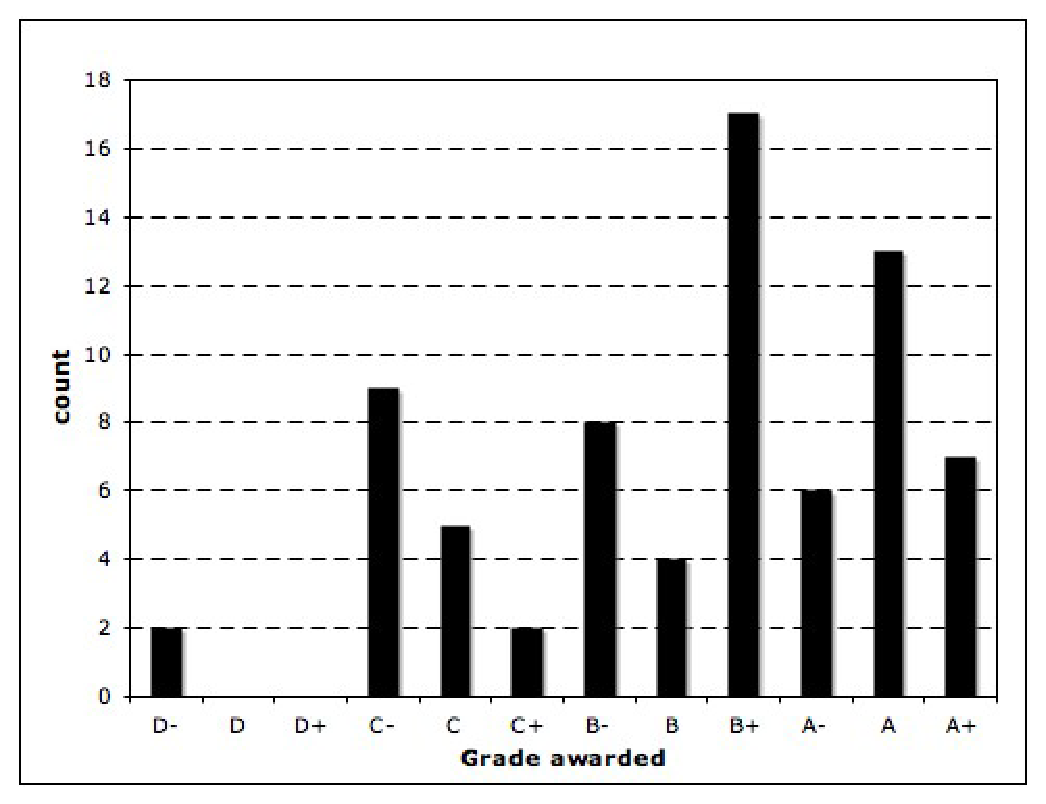
\includegraphics [scale=0.01] {grades.eps}
}
\caption{Distribution of grades for lab reports}
\label{grades_histo}
\end{center}
\end{figure}

\begin{figure}[htb]
  \centering
\resizebox{0.8\textwidth}{!}{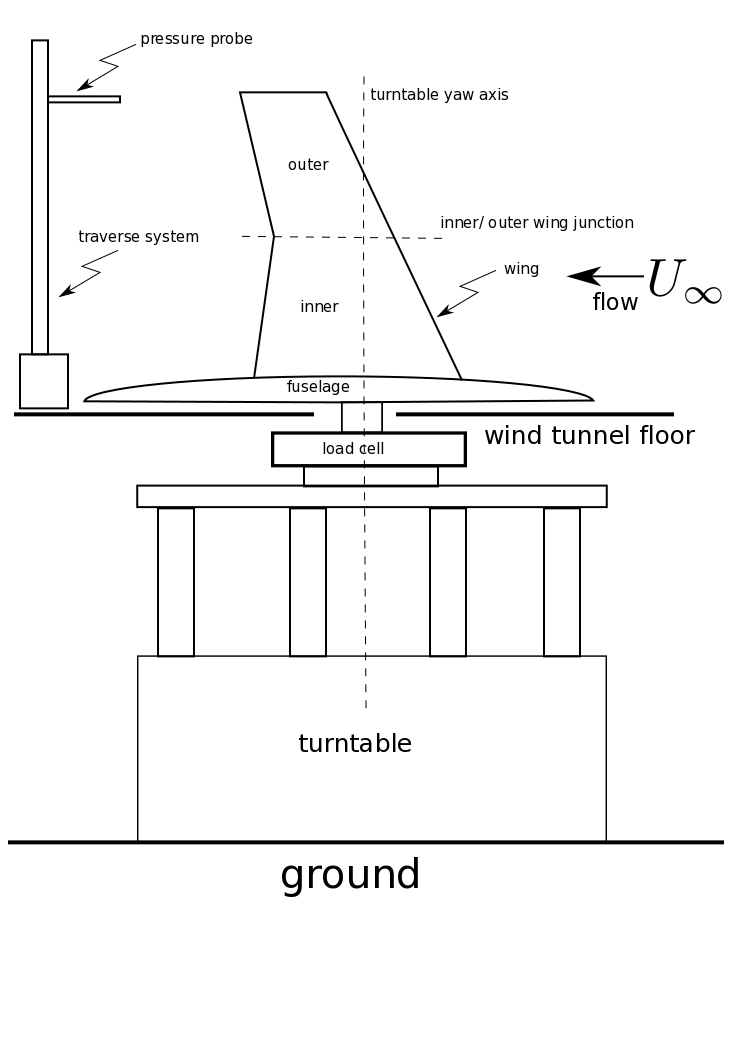
\includegraphics{wing_in_tunnel.png}}
\caption{Schematic diagram of wing model in the wind tunnel. The diagram was sketched using inkscape.}
\label{wingtunnel}
\end{figure}


\begin{figure}[htp]
\centering
(a) 0 degrees \hspace{5cm} (b) 5 degrees
\resizebox{1.0\textwidth}{!}{%
  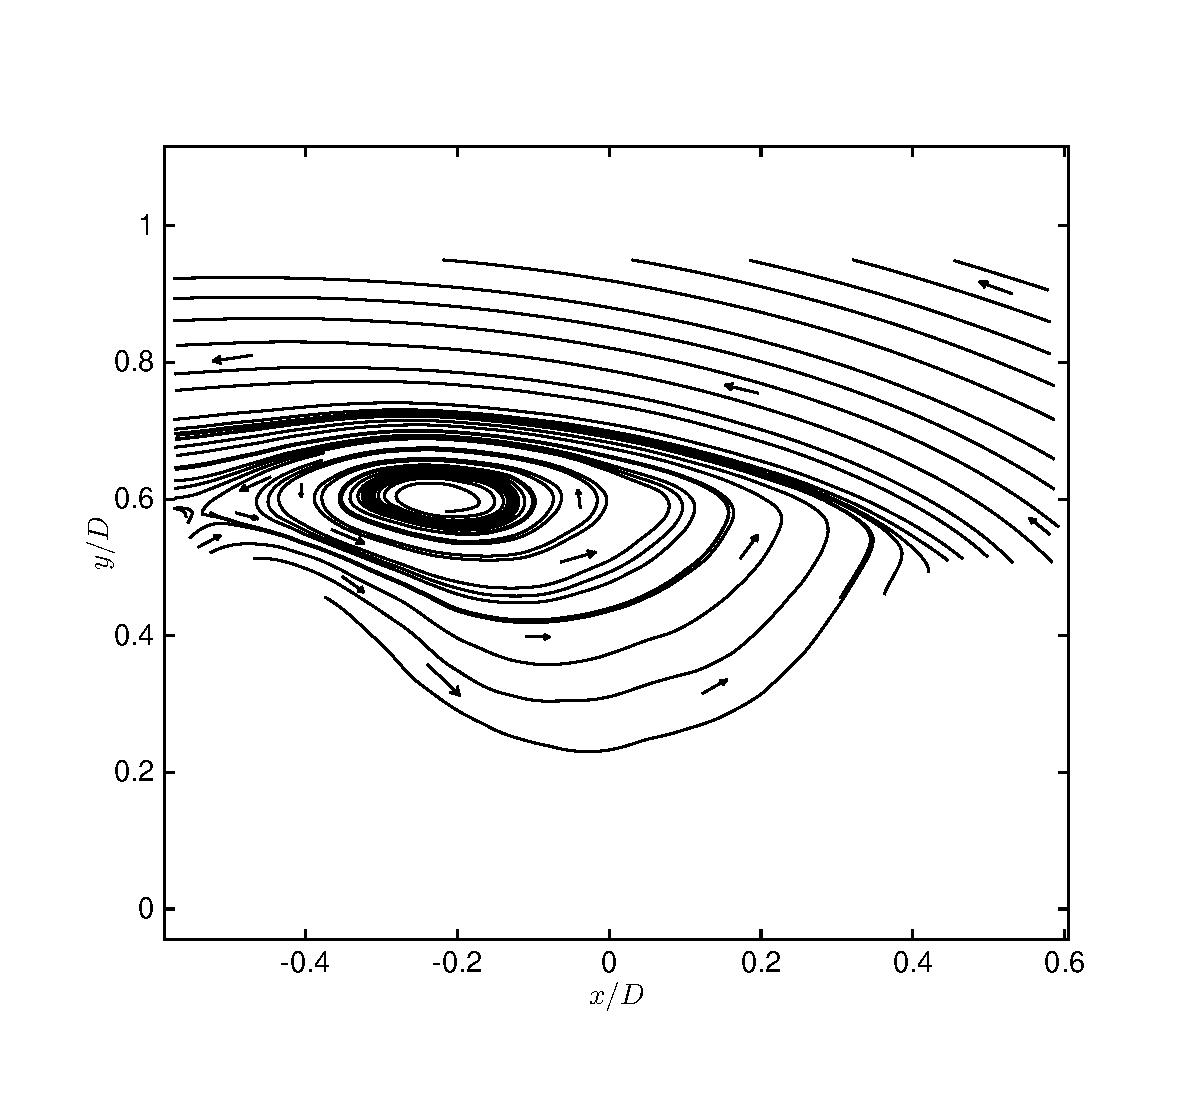
\includegraphics{0degslines.eps}
    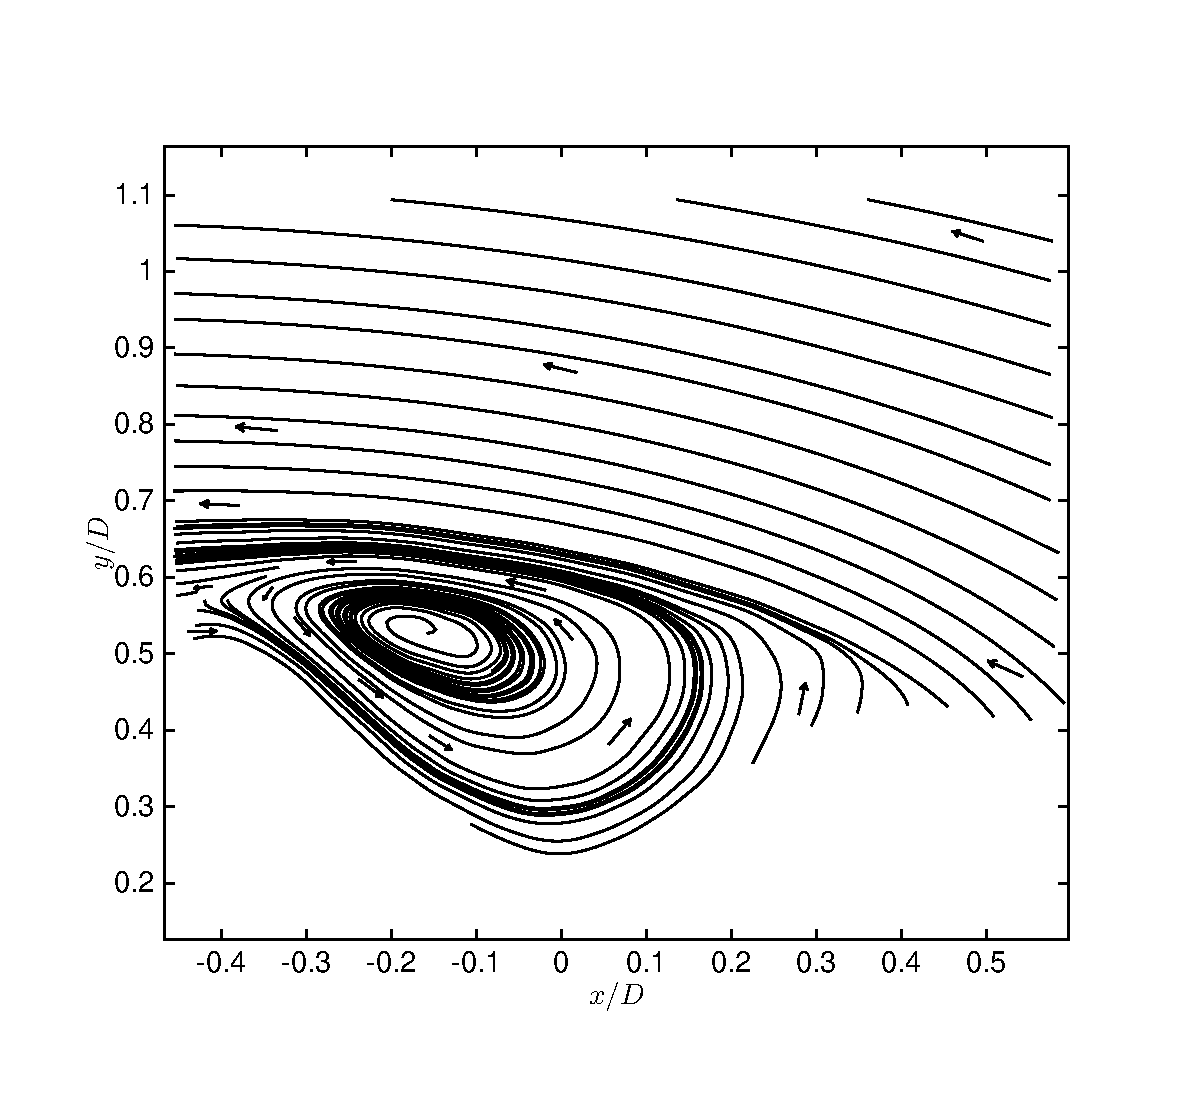
\includegraphics{5degslines.eps}
  }
 \caption{Mean flow streamlines. Note the sub-captions for each frame (a) and (b).}
\label{slines} 
\end{figure}



%
%\begin{figure}
% (a) interaction case i2  \hspace{3cm} (b) interaction case i3
% 
%\resizebox{1.0\textwidth}{!}{%
%		\includegraphics{apr13_fore_2p5_17_vort.eps}
%		\includegraphics{apr13_fore_2p5_59_vort.eps}
%		}
%(c) interaction case i5
%
%\resizebox{0.5\textwidth}{!}{%
%		\includegraphics{apr11_2p5_17_vort.eps}
%		}
%\caption{Evolution of vorticity field during lower surface interaction (non-dimensional data shown). See Table 1. for details. Frames (a), (b) and (c) show typical vorticity plots as the vortex moves aft.}
%\label{ls_interaction_vort}
%\end{figure}



\end{document}